\documentclass[a4paper,11pt]{article}
%\pdfoutput=1 % if your are submitting a pdflatex (i.e. if you have
             % images in pdf, png or jpg format)
\usepackage{graphicx}
\usepackage{jcappub} % for details on the use of the package, please
                     % see the JCAP-author-manual

%\usepackage[T1]{fontenc} % if needed



\title{One Student One Laptop(OSOL)}


%% %simple case: 2 authors, same institution
 \author{Dennis Goeken}
 \author{and Han Yang}

\affiliation{IKAROS Shared Team, Riverty Group GmbH}

% e-mail addresses: one for each author, in the same order as the authors
\emailAdd{dennis.goeken@riverty.com}
\emailAdd{han.yang@riverty.com}

%\abstract{Abstract...}

\begin{document}
\maketitle
\flushbottom

\section{What is One Student One Laptop(OSOL)?}
In One Student One Laptop(OCOL), we collect denoted out-of-date IT equipments, such as Laptop, Tablet, LCD Monitor, Mounse, Keyboard. Then we do cleaning and disinfection. Then we will reset this Laptop/Tablet to factory setting. Then if possible, we will install ChromeOS Flex on this Laptop/Tablet. Then we rent these IT equipments to the students in the developing countries to help their learning and developing. 


\section{Why OSOL?}

\subsection{Education would change one life}
\href{https://www.unesco.org/en/education}{Education would change one life}

Education is more than just learning facts and skills. It is a transformative process that can change your life and the lives of others. Education can help you discover your passions, develop your talents, and achieve your goals. Education can also empower you to make a positive difference in the world, by contributing to social change, economic growth, and human development.

But not everyone has access to quality education. Millions of people around the world face barriers such as poverty, discrimination, conflict, and lack of resources. These challenges prevent them from reaching their full potential and fulfilling their purpose.\cite{education-change-life-world}

What is Education and Why is it Important?

Education is the process of acquiring knowledge, skills, values, and attitudes that enable people to learn, grow, and thrive. Education can take many forms, such as formal schooling, informal learning, vocational training, lifelong learning, etc. Education can also cover various subjects, such as literacy, numeracy, science, arts, culture, etc.

Education is important for many reasons. Here are some of them:

Education can improve your health and well-being. Studies have shown that education can reduce the risk of diseases, increase life expectancy, improve mental health, and enhance self-esteem.
Education can increase your income and employment opportunities. Studies have shown that education can boost your productivity, creativity, and innovation. Education can also help you access better jobs, earn higher wages, and escape poverty.
Education can enhance your social and civic participation. Studies have shown that education can foster your critical thinking, communication, and collaboration skills. Education can also help you develop your values, beliefs, and identity. Education can also enable you to participate in democratic processes, such as voting, volunteering, and activism.
Education can promote peace and justice. Studies have shown that education can reduce violence, conflict, and extremism. Education can also help you understand different perspectives, respect diversity, and promote human rights.

How Education Can Empower Individuals and Communities

Education is not only beneficial for individuals but also for communities. Education can empower people to take charge of their own lives and contribute to the common good. Here are some examples of how education can empower individuals and communities:

Education can empower children and youth. Children and youth are the future of our society. They have the potential to shape the world for the better. But they also face many challenges, such as malnutrition, disease, child labor, child marriage, etc. By providing them with education, we can help them grow up healthy, happy, and safe. Education can also help them develop their cognitive, emotional, social, and physical abilities. Education can also enable them to express their opinions, aspirations, and creativity.
Education can empower marginalized groups. Marginalized groups are those who are excluded, ignored or discriminated against because of their ethnicity, religion, disability, sexual orientation, etc. By providing them with education, we can help them overcome these challenges and achieve social inclusion. Education can also help them develop their identity, dignity, and respect. Education can also enable them to access their rights, opportunities, and resources.
Education can empower communities. Communities are groups of people who share a common interest, location, or culture. By providing them with education, we can help them improve their quality of life, well-being, and resilience. Education can also help them develop their social capital, collective action, and problem-solving skills. Education can also enable them to participate in community development, environmental protection, and conflict resolution.

\subsection{Internet helped Education}
The internet contains a wealth of knowledge that can be accessed anytime and anywhere. 

The importance of Internet access to students
90% of the information on the Internet has been created in the past year. Having access to the Internet allows students to keep up with information that might not make it into textbooks or become outdated by the time it becomes available in a traditional format.

Having access to this information empowers students to take charge of their education, and the research backs that up. Students with access to internet-capable devices tend to score higher on tests. Other studies showed that discipline issues decreased when students could use technology to help with their studies. \cite{why-student-must-internet-access}

\subsubsection{Relevant Information Present on the Internet} \cite{internet-beneficial-students}
When the internet was still in its inception, finding reliable information was a much more difficult task than today.

Before the internet, people had to rely on traditional sources such as libraries and encyclopedias for research.

Libraries were the only places where people could find the information they were looking for, and researching could take hours, or days, depending on the topic.

This could be quite time-consuming and tedious. Fortunately, the internet has revolutionized the way students learn.

With the click of a button, students have access to an unprecedented amount of information, resources, and tools to help them with their studies.

This saves a lot of time and energy.
\subsubsection{Developing Communication and Connectivity}
Some students need to connect virtually with others to collaborate on projects and assignments. With an internet service provider, students can communicate online with their classmates and teachers.

The internet has enabled students to connect with other students and teachers from all over the world.

This has allowed students to work with people from different languages, cultures, backgrounds, and experiences, which can be incredibly valuable for their learning.

The internet has also allowed for easier and more efficient communication.

Before the internet, students had to rely on traditional methods such as mail, phone calls, or in-person meetings.

This could be costly and time-consuming. With the internet, students can instantly connect with their peers and teachers with both the written word and by video all without traveling.

This lets students stay connected with their classmates and teachers and receive feedback quickly.

\subsubitem{Access to Educational Resources}
Reliable internet connectivity opens up an expansive world of educational resources that simply aren’t available in traditional settings. Students can access extensive online libraries filled with thousands of e-books, academic journals, and scholarly articles. Major platforms offer video lectures from experts around the globe, which can introduce new perspectives and teaching methods that enhance understanding.

Interactive learning platforms like virtual labs, simulations, and educational games provide hands-on experience in subjects that would otherwise be difficult to visualize or practice in a physical classroom. This access enables students to delve deeper into topics of interest, explore complex concepts through multimedia content, and stay current with the latest academic research and innovations.

\subsubsection{Collaborative Projects}
Reliable internet makes it possible for students to work together effectively on group projects, even when they are miles apart. Cloud-based tools like Google Drive, Dropbox, and Microsoft OneDrive allow team members to co-edit documents in real time, share files instantly, and keep track of project updates.

\subsubsection{Access to Online Courses and Certifications}
The digital age has democratized education by providing access to a plethora of online courses and certification programs offered by prestigious institutions around the world. With reliable internet, students can enroll in these courses to gain specialized skills, earn certifications, and enhance their academic credentials.

Flexible scheduling and self-paced learning options make it easier to balance these courses with regular schoolwork or part-time jobs. Additionally, many online platforms offer interactive elements like quizzes, peer reviews, and discussion boards, which enrich the learning experience and foster a global community of learners.

\subsubsection{Flexibility in Learning Environments}
A strong internet connection provides unprecedented flexibility in where and how students learn. No longer confined to traditional classrooms, students can now access their coursework from any location, whether it’s the comfort of their home, a quiet café, or even while traveling. This flexibility supports diverse learning styles and allows students to create study environments that suit their personal preferences and needs.

For those balancing education with other responsibilities, such as part-time jobs or family commitments, this adaptability is invaluable. It also enables self-paced learning, where students can revisit lectures and take extra time to master difficult concepts.


Imagine a student in a remote area accessing virtual field trips to museums, historical landmarks, and scientific labs worldwide. This digital exploration fosters curiosity and broadens horizons, enabling students to experience diverse cultures and global perspectives without leaving their homes. These experiences cultivate a sense of global citizenship and empathy—essential qualities in our interconnected world.



\subsection{GPT helped Education}

\section{Related Resouces}
\subsection{One Laptop per Child}
\url{https://en.wikipedia.org/wiki/One\_Laptop\_per\_Child}

\subsection{World Computer Exchange}
\url{https://en.wikipedia.org/wiki/World\_Computer\_Exchange}

\subsection{Windows 11 24H2 update}

\subsection{UNESCO}

Education transforms lives and is at the heart of UNESCO’s mission to build peace, eradicate poverty and drive sustainable development. It is a human right for all throughout life. The Organization is the only United Nations agency with a mandate to cover all aspects of education. It has been entrusted to lead the Global Education 2030 Agenda through Sustainable Development Goal 4.  

UNESCO provides global and regional leadership in education, strengthens education systems worldwide and responds to contemporary global challenges through education with gender equality as an underlying principle. Its work encompasses quality educational development from pre-school to higher education and beyond. \cite{unesco-education-transforms-lives}

\section{What Riverty and Bertelsmann will get?}
The Advertisement effect during the whole process with tiny cost.

\section{How OLPC?}

\subsection{one IT equipment lifecycle}
\begin{figure}
	\centering
	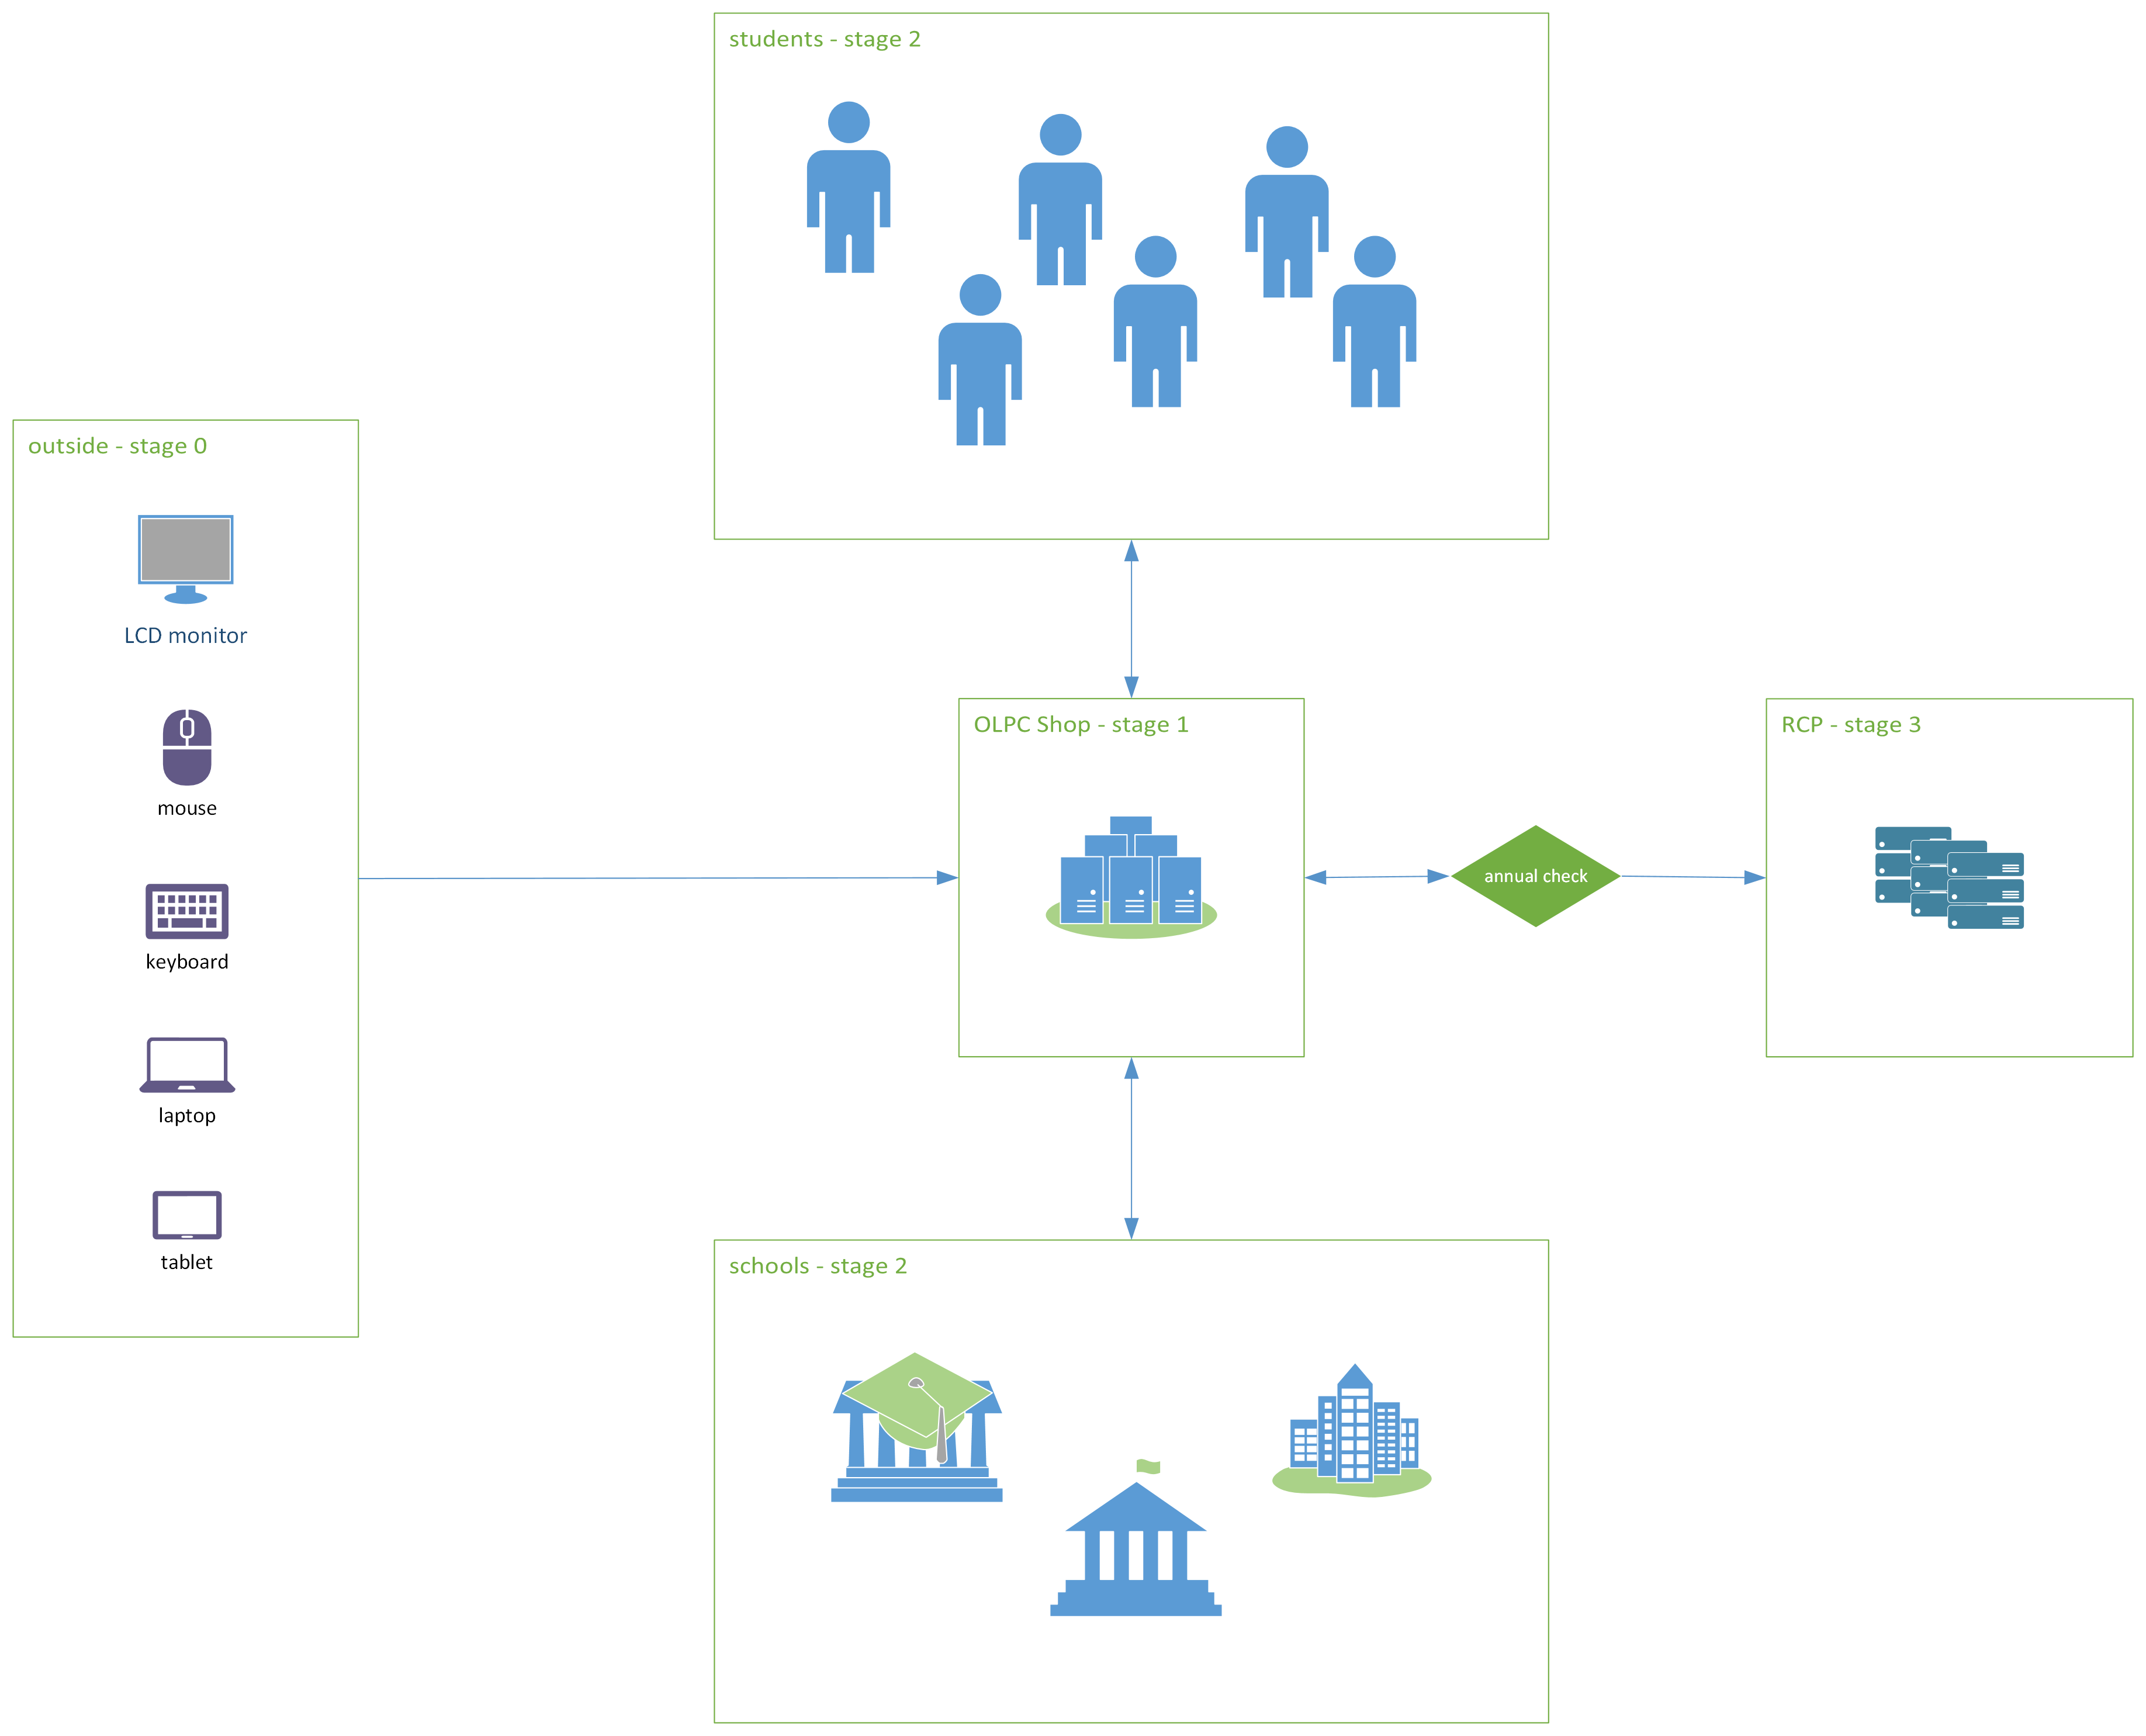
\includegraphics[width=0.9\linewidth]{olpc-rcp}
	\caption{IT equipments lifecycle}
	\label{fig:olpc-rcp}
\end{figure}


\subsubsection{OLPC IT equipment stages}
\begin{enumerate}
	\item Stage 0 - outside OLPC
	\item Stage 1 - stay in OLPC Shop
	\item Stage 2 - stay in student: less Grade4(10 years old) use Tablet, from Grade5(11 years old) start use laptop, start coding.
	\item Stage 3 - stay in RCP
\end{enumerate}	

\subsection{use 2D barcode to trace the equipement stage}

\subsection{IT equipment score}

\subsection{Annual check}

	
\subsection{OLPC Tracer - OLPC Data Management System}
\subsubsection{OLPC-T Architecture}
\begin{figure}
	\centering
	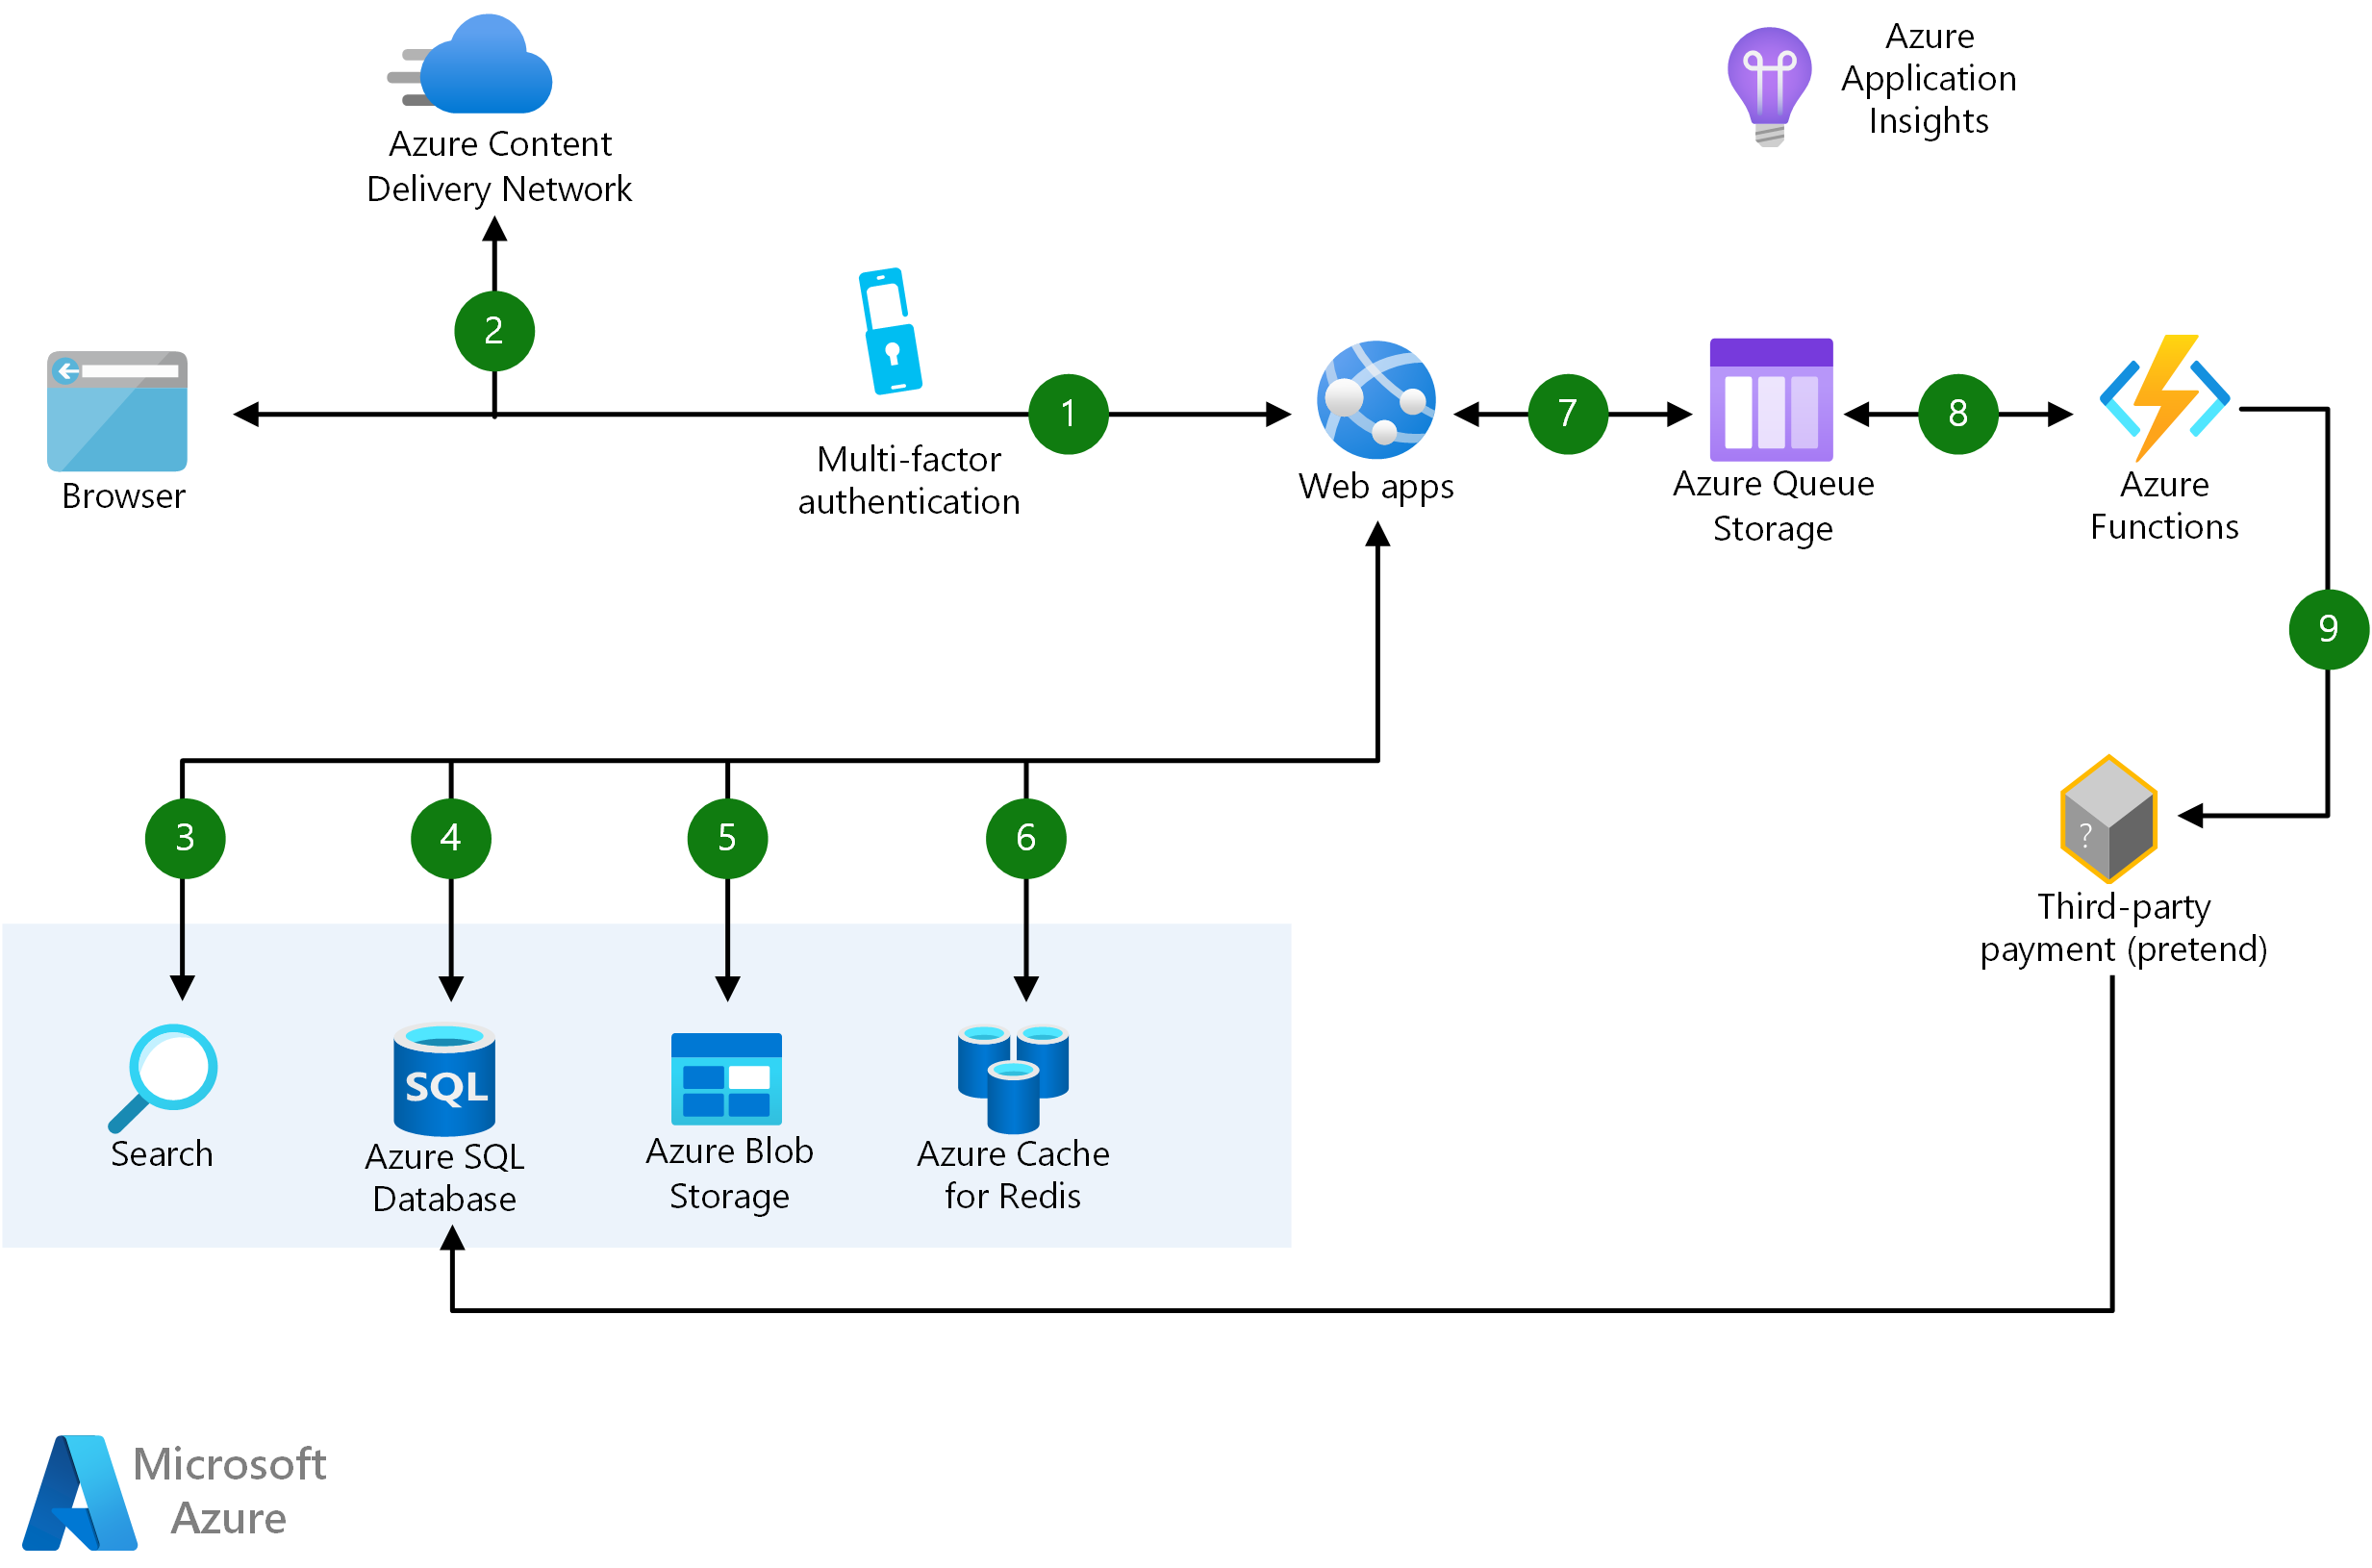
\includegraphics[width=0.9\linewidth]{scalable-ecommerce-web-app}
	\caption{OLPC Tracer Draft Architecture}
	\label{fig:scalable-ecommerce-web-app}
\end{figure}


\subsubsection{OLPC-T Database - relation database - MS Azure SQL Server}
\subsubsection{OLPC-T API - MS Azure Function }
\subsubsection{OLPC-T API Management }
\begin{figure}
	\centering
	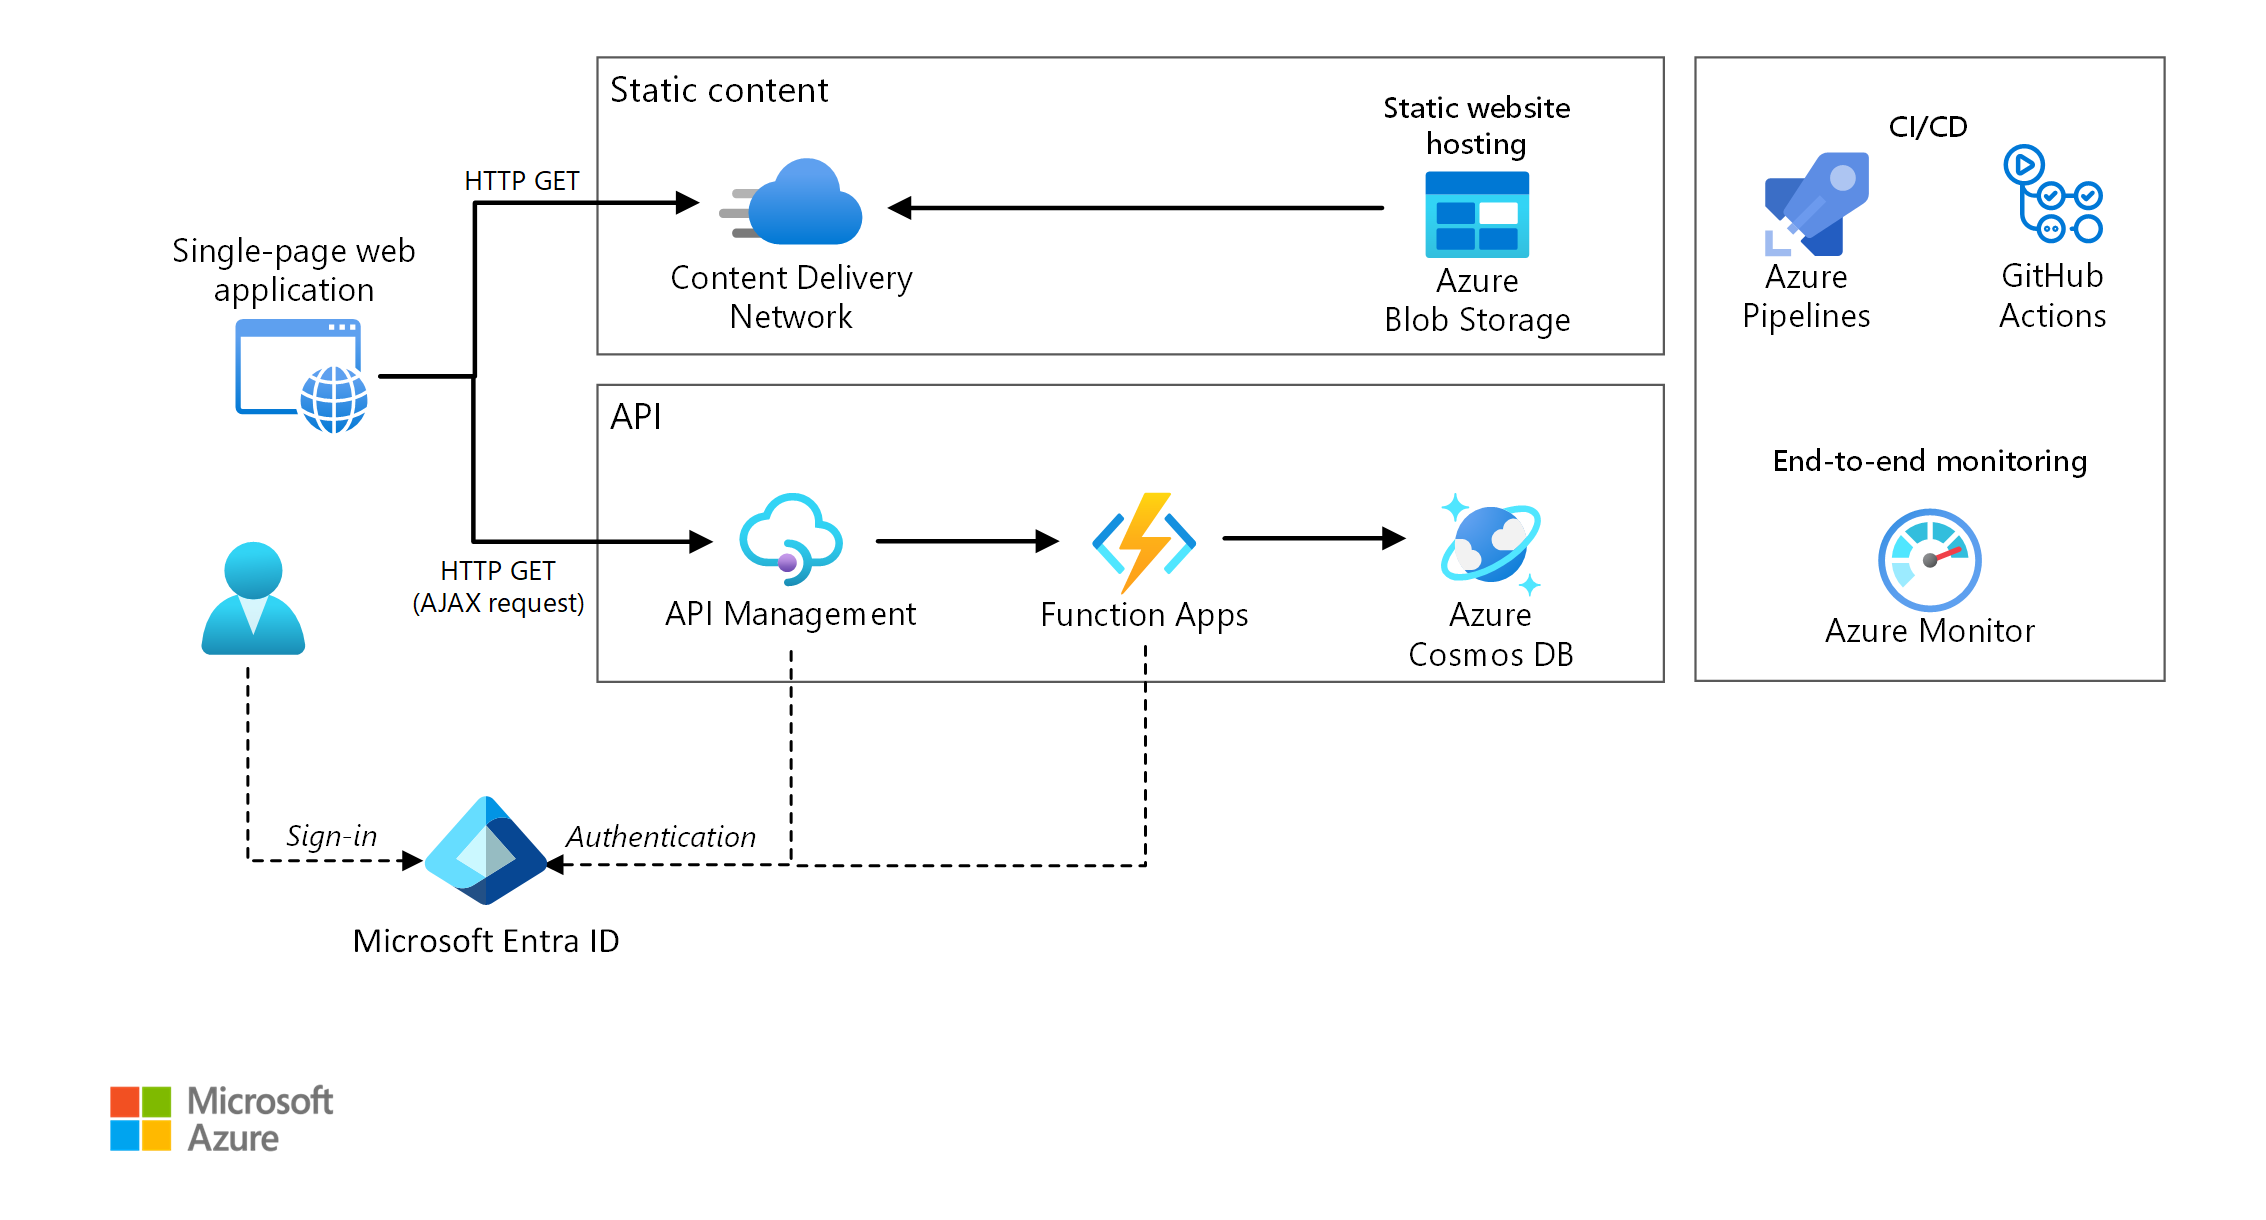
\includegraphics[width=0.9\linewidth]{serverless-web-app}
	\caption{MS Azure Serverless Architecture}
	\label{fig:serverless-web-app}
\end{figure}
\subsubsection{OLPC-T GUI}
\begin{enumerate}
	\item Multi-Platform - Desktop, Mobile, Web
	\item Multi-Platform - Flutter/Dart
	\item Input
	\item Search
	\item Scan 2D barcode
	\item ChatBot
\end{enumerate}



\subsection{Riverty Computer Pool(RCP)}
\begin{enumerate}
	\item RCC-abstract IO
	\item RCC-robust
	\item RCC-decentralization
	\item RCC-duplication and backup - data/process holographic : even $1/3$ computers are fail. $99.999\%$ data and computing process should be OK.
	\item RCC-hot plugging in Computer level
	\item RCC-AI based - ChatBot
\end{enumerate}


\section{Schedule}
\subsection{Step 1}
\begin{enumerate}
\item Just one place to store these out of date IT equipment.
\item Another guy to monitor and confirm each other with me.
\end{enumerate}

\appendix
\section{Why we use queue in OLPC-T architecture?}
\begin{enumerate}
	\item Decoupling
	\begin{itemize}
		\item Purpose: Queues act as a buffer between the API and the downstream services, such as databases or processing logic.
		\item Benefit: This ensures that the API can handle incoming requests without being directly tied to the speed or availability of the downstream services.
		\item Example: A user uploads data via an API, which places a message in a queue. The processing of the data happens asynchronously, allowing the API to quickly respond to the user.
	\end{itemize}
	\item Scalability
	\begin{itemize}
		\item Purpose: In serverless environments, the workload can spike unpredictably. A queue helps handle bursts of traffic by storing messages until they can be processed.
		\item Benefit: This allows your application to scale gracefully. For instance, Azure Functions or Logic Apps can process messages from the queue as they scale up or down automatically.
		\item Example: During high traffic, the queue can hold requests until Azure Functions has enough capacity to process them.
	\end{itemize}
	\item Reliability and Resilience
	\begin{itemize}
		\item Purpose: Queues ensure that no messages are lost, even if downstream services fail or experience downtime.
		\item Benefit: This helps in building fault-tolerant systems where messages are retried or processed later when the system recovers.
		\item Example: A queue can store order details submitted via an API. If the order-processing system crashes, the orders remain safe in the queue until the system is back online.
	\end{itemize}
	\item Throttling and Load Management
	\begin{itemize}
		\item Purpose: Queues help control the rate at which messages are processed by downstream services, preventing overload.
		\item Benefit: This protects the system from performance degradation or failures due to resource exhaustion.
		\item Example: The API can accept thousands of requests per second, but the backend may process only a hundred at a time. The queue enforces this limit.
	\end{itemize}
	\item Asynchronous Processing
	\begin{itemize}
		\item Purpose: Many tasks do not need to be performed immediately and can be handled in the background.
		\item Benefit: This improves the user experience by providing faster responses from the API and ensures better resource utilization.
		\item Example: An image-processing API can accept uploads quickly and push them to a queue. Processing, resizing, and storing the images happens asynchronously.
	\end{itemize}
	\item Retry and Dead-Letter Handling
	\begin{itemize}
		\item Purpose: Queues often support retries and dead-letter queues (DLQs) for failed messages.
		\item Benefit: If a message cannot be processed, it can be retried a set number of times, and if it still fails, it is moved to a DLQ for further investigation.
		\item Example: A payment processing API ensures no transaction request is lost. Failed requests are retried or stored in a DLQ.
	\end{itemize}
	\item Integration with Azure Services
	\begin{itemize}
		\item Azure provides built-in support for queues with services like Azure Queue Storage and Azure Service Bus. These services integrate seamlessly with Azure serverless components such as:
		\begin{itemize}
			\item Azure Functions: Triggered by queue messages to process tasks.
			\item Azure Logic Apps: Orchestrates workflows using queue messages.
			\item Azure Event Grid: Enables event-driven processing.
		\end{itemize}
	\end{itemize}
	
	\item Real-World Scenario
	For an e-commerce API:
	\begin{enumerate}
		\item A user places an order via the API.
		\item The order details are added to a queue.
		\item Downstream services like inventory checking, payment processing, and order confirmation process the queue messages asynchronously.
		\item If any service fails, the queue retains the message for retry or troubleshooting.
	\end{enumerate}
\end{enumerate}


%\begin{thebibliography}{99}

	%\bibitem{education-change-life-world}
	%\emph{How Education Can Change Your Life and the World: A Guide to Unlocking Your Potential and Fulfilling Your Purpose}. In {Araceli Aid Foundation}.  %\url{https://araceliaidfoundation.org/education/how-education-can-change-your-life-and-the-world-a-guide-to-unlocking-your-potential-and-fulfilling-your-purpose/}

	% Please avoid comments such as "For a review'', "For some examples",
	% "and references therein" or move them in the text. In general,
	% please leave only references in the bibliography and move all
	% accessory text in footnotes.
	
	% Also, please have only one work for each \bibitem.

%\end{thebibliography}

\bibliography{reference}{}
\bibliographystyle{plainurl}

\end{document}